%%% Econ712: Macroeconomics I
%%% Fall 2020
%%% Danny Edgel
%%%
% Due on Canvas Wednesday September 18, 11:59pm Central Time
%%%

%%%
%							PREAMBLE
%%%

\documentclass{article}

%%% declare packages
\usepackage{amsmath}
\usepackage{amssymb}
\usepackage{array}
\usepackage{bm}
\usepackage{changepage}
\usepackage{centernot}
\usepackage{graphicx}
\usepackage{fancyhdr}
	\fancyhf{} % sets both header and footer to nothing
	\renewcommand{\headrulewidth}{0pt}
    \rfoot{Edgel, \thepage}
    \pagestyle{fancy}
	
%%% define shortcuts for set notation
\newcommand{\N}{\mathbb{N}}
\newcommand{\Z}{\mathbb{Z}}
\newcommand{\R}{\mathbb{R}}
\newcommand{\Q}{\mathbb{Q}}
\newcommand{\lmt}{\underset{x\rightarrow\infty}{\text{lim }}}
\newcommand{\neglmt}{\underset{x\rightarrow-\infty}{\text{lim }}}
\newcommand{\zerolmt}{\underset{x\rightarrow 0}{\text{lim }}}
\newcommand{\usmax}{\underset{1\leq k \leq n}{\text{max }}}

%%% define column vector command (from Michael Nattinger)
\newcount\colveccount
\newcommand*\colvec[1]{
        \global\colveccount#1
        \begin{pmatrix}
        \colvecnext
}
\def\colvecnext#1{
        #1
        \global\advance\colveccount-1
        \ifnum\colveccount>0
                \\
                \expandafter\colvecnext
        \else
                \end{pmatrix}
        \fi
}

%%% define function for drawing matrix augmentation lines
\newcommand\aug{\fboxsep=-\fboxrule\!\!\!\fbox{\strut}\!\!\!}

\makeatletter
\let\amsmath@bigm\bigm

\renewcommand{\bigm}[1]{%
  \ifcsname fenced@\string#1\endcsname
    \expandafter\@firstoftwo
  \else
    \expandafter\@secondoftwo
  \fi
  {\expandafter\amsmath@bigm\csname fenced@\string#1\endcsname}%
  {\amsmath@bigm#1}%
}


%________________________________________________________________%

\begin{document}

\title{	Problem Set \#2 }
\author{ 	Danny Edgel 					\\ 
			Econ 712: Macroeconomics I		\\
			Fall 2020						\\
		}
\maketitle\thispagestyle{empty}

%%%________________________________________________________________%%%

\textit{Collaborated with Sarah Bass, Emily Case, Michael Nattinger, and Alex Von Hafften}


%%%________________________________________________________________%%%

\section*{Question 1}
We are given:
\begin{align*}
	k_{t+1} &= f(k_t)+(1-\delta)k_t-c_t		\\
	\beta u'(c_{t+1}) &= \frac{u'(c_t)}{1-\delta+f'(k_{t+1})}
\end{align*}
Where $f(k)=zk^\alpha$ and $u(c)=\text{log}(c)$.

\begin{enumerate}
	\item Let $k_{t+1}=k_t=\overline{k}$ and $c_{t+1}=c_t=\overline{c}$. Then:
		\begin{align*}
			&\overline{k}=z\overline{k}^\alpha+(1-\delta)\overline{k} - \overline{c}	
			& \beta \frac{1}{\overline{c}}=\left(\frac{1}{\overline{c}}\right)\left(\frac{1}{1-\delta+\alpha z \overline{k}^{\alpha-1}}\right)				\\
			&\overline{c}=z\overline{k}^\alpha-\delta\overline{k}	
			& \frac{1}{\beta}= 1-\delta+\alpha z \overline{k}^{\alpha-1} 	\\
			& 	& \overline{k}^{\alpha-1} = \frac{\frac{1}{\beta}+\delta-1}{\alpha z}		\\
			& \overline{c}=z
				\left(\frac{\frac{1}{\beta}+\delta-1}{\alpha z}
						\right)^{\frac{\alpha}{\alpha-1}}
				-\delta\left(
							\frac{\frac{1}{\beta}+\delta-1}{\alpha z}
							\right)^{\frac{1}{\alpha-1}} 	
				& \overline{k} = \left(
									\frac{\frac{1}{\beta}+\delta-1}{\alpha z}
									\right)^{\frac{1}{\alpha-1}}	
		\end{align*}
		Inputting the parameters provided in the question ($z=1$, $\alpha=0.3$, $\delta=0.1$, and $\beta=0.97$) yields $\overline{k}\approx3.2690$ and $\overline{c}\approx 1.0998$.\footnote{See the attached file, edgel\_ps2.R, for this computation.}
		
	\item The steps for linearizing the system as follows.
		\begin{enumerate}
			\item The equations for $k_{t+1}$ and $c_{t+1}$ can be rewritten as:
				\begin{align*}
					k_{t+1} &= g(k_t,c_t) = zk_t^\alpha + (1-\delta)k_t-c_t \\
					c_{t+1} &= h(k_t,c_t) = \beta c_t\left(1-\delta+\alpha z(zk_t^\alpha + (1-\delta)k_t-c_t)^{\alpha-1}\right)
				\end{align*}
				
			\item The Jacobian matrix is:
				\[
					\begin{pmatrix}
						\alpha zk_t^{\alpha-1}+1-\delta 	& -1 					\\ 
						dc_{t+1}/dk_t					& dc_{t+1}/dc_t
					\end{pmatrix}
				\]
				Where:
				\begin{align*}
					\frac{dc_{t+1}}{dk_t} &= \beta(\alpha-1)\alpha z c_t(z k_t^\alpha + (1-\delta)k_t - c_t)^{\alpha-2}(\alpha z k_t^{\alpha-1}+1-\delta)	\\
					\frac{dc_{t+1}}{dc_t} &= \beta(1-\delta+\alpha z(zk_t^\alpha+(1-\delta)k_t-c_t)^{\alpha-1})-\beta(\alpha-1)\alpha z c_t(zk_t^\alpha+(1-\delta)k_t-c_t)^{\alpha-2}
				\end{align*}
				
			\item Define:
				\[
					\colvec{2}{\widetilde{k}_{t+1}}{\widetilde{c}_{t+1}} = J\colvec{2}{\widetilde{k}_{t}}{\widetilde{c}_{t}}
					=J\colvec{2}{k_t-\overline{k}}{c_t-\overline{c}}
				\]
		\end{enumerate}
		
	\item Using the R code provided with this assignment, I computed the Jacobian's steady-state eigenvalues as $1.2060$ and $0.8548$. Since $|\lambda_1|>1$ and $|\lambda_2|<1$, this system has a saddle path. Staying on the saddle path means moving along the stable eigenvector(i.e. the vector associated with the eigenvalue with an absolute value less than one). In this case, the stable eigenvalue is $v_1=(0.9850,0.1725)$, so the slope of the saddle path is $\frac{0.1725}{0.9850}=0.1751$.
	
	\item The diagram below shows how the system evolves after a permanent, unexpacted productivity shock. The dashed blue line displays the (approximate, drawn in Paint) saddle path for the initial productivity level, where the blue dot indicates the steady state level of capital and consumption. The red dot and dashed red line display the same for the new captial level. In the period of the productivity shock, consumption jumps from the initial productivity's steady state to the level of consumption that matches the fixed capital level's consumption along the new saddle path (indicated on the chart by the green point). In the periods that follow, consumption follows the saddle path (shown in green) until it reaches the new steady state.
		\begin{center}
			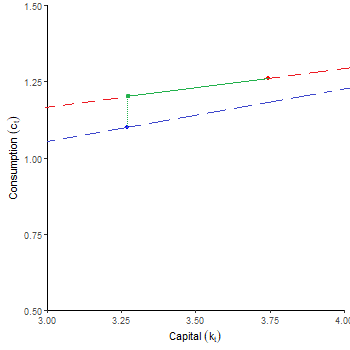
\includegraphics[scale=1]{problem1_phaseplot_edited.png}
		\end{center}
		
	\item Below, I follow the steps described in the problem:
		\begin{enumerate}
			\item In the R code provided, I compute:
				\begin{align*}
					&\colvec{2}{\overline{k}'}{\overline{c}'} = \colvec{2}{3.7458}{1.2602} &J=\begin{pmatrix} 1.0190 & -1 \\ -0.0280 & 1.0299 \end{pmatrix}
				\end{align*}
				
			\item Let $J=E\Lambda E^{-1}$, where $\Lambda$ is the diagonal matrix of $J$'s eigenvalues. Then, from using the R code provided, we can derive:
				\[
					J=E\Lambda E^{-1}\begin{pmatrix} 0.9854 & -0.9871 \\ -0.1704 & -0.1510 \end{pmatrix}\begin{pmatrix} 1.1920 & 0 \\ 0 & 0.8570 \end{pmatrix}\begin{pmatrix} 0.4909 & -3.0292 \\ -0.5230 & -3.0238 \end{pmatrix}
				\]
				Now, let:
				\[
					\colvec{2}{\widehat{k}_t}{\widehat{c}_t} = E^{-1}\colvec{2}{k_t}{c_t}
				\]
				
			\item Using the definition from (b) of $(\hat{k}_t,\hat{c}_t)$, we can solve:
				\begin{align*}
					\colvec{2}{k_{t+1}}{c_{t+1}} 						&= J\colvec{2}{k_t}{c_t}	\\
					E\colvec{2}{\widehat{k}_{t+1}}{\widehat{c}_{t+1}} 	&= (E\Lambda E^{-1})\left(\colvec{2}{\widehat{k}_t}{\widehat{c}_t}\right) \\
					\colvec{2}{\widehat{k}_{t+1}}{\widehat{c}_{t+1}} 	&= (E^{-1}E)\Lambda(E^{-1}E)\colvec{2}{\widehat{k}_t}{\widehat{c}_t} \\
					\colvec{2}{\widehat{k}_{t+1}}{\widehat{c}_{t+1}} 	&= \Lambda\colvec{2}{\widehat{k}_t}{\widehat{c}_t} \\
					\colvec{2}{\widehat{k}_{t+1}}{\widehat{c}_{t+1}} 	&= \colvec{2}{\lambda_1\widehat{k}_t}{\lambda_2\widehat{c}_t}
				\end{align*}
				Thus,
				\[
					\colvec{2}{\widehat{k}_t}{\widehat{c}_t}  = \colvec{2}{\lambda_1^t\widehat{k}_0}{\lambda_2^t\widehat{c}_0}
				\]
				Where $\lambda_1=1.1920$ and $\lambda_2=0.8570$. Since $|\lambda_1|>1$, any non-explosive solution requires that $\widehat{k}_0=0$. Thus, rewriting in terms of $(k_t,c_t)$, we have:
				\begin{align*}
					\colvec{2}{k_t}{c_t} &= E\colvec{2}{\widehat{k}_t}{\widehat{c}_t} \\
					\colvec{2}{k_t}{c_t} &= \begin{pmatrix} e_{11} & e_{12} \\ e_{21} & e_{22} \end{pmatrix} \colvec{2}{\lambda_1^t\widehat{k}_0}{\lambda_2^t\widehat{c}_0} \\
					\colvec{2}{k_t}{c_t} &= \colvec{2}{e_{11}\lambda_1^t\widehat{k}_0+e_{12}\lambda_2^t\widehat{c}_0}{e_{21}\lambda_1^t\widehat{k}_0+e_{22}\lambda_2^t\widehat{c}_0} \\
					\colvec{2}{k_t}{c_t} &= \colvec{2}{e_{12}\lambda_2^t\widehat{c}_0}{e_{22}\lambda_2^t\widehat{c}_0}
				\end{align*}
				
			\item Our initial condition at $t_0$ is $(k_{t_0},c_{t_0})$, and our boundary condition is $(\overline{k}',\overline{c}')$, where $k_{t_0}=\overline{k}$ and we need to solve for $c_{t_0}$. This enables us to solve for the general solution:
				\begin{align*}
					\overline{k} 				&= e_{12}\lambda_2^5\widehat{c}_0+\overline{k}'			 	\\
					\widehat{c}_0				&=\frac{\overline{k}-\overline{k}'}{e_{12}\lambda_2^5} 		\\
					c_t^g 						&=e_{22}\lambda_2^t\left(\frac{\overline{k}-\overline{k}'}{e_{12}\lambda_2^5}\right)+\overline{c} \\
					\colvec{2}{k_t^g}{c_t^g} 	&= \colvec{2}{e_{12}\lambda_2^t\left(\frac{\overline{k}-\overline{k}'}{e_{12}\lambda_2^5}\right)+\overline{k}'}{e_{22}\lambda_2^t\left(\frac{\overline{k}-\overline{k}'}{e_{12}\lambda_2^5}\right)+\overline{c}}
				\end{align*}
				
			\item Using the known values of $E$ and the steady states, listed in earlier points, the provided R code calculated $k_t$ and $c_t$ for $t=1,...,20$. The charts below show the evolution of each value over time, with the pre- and post-shock steady stated indicated by dashed lines.
				\begin{center}
					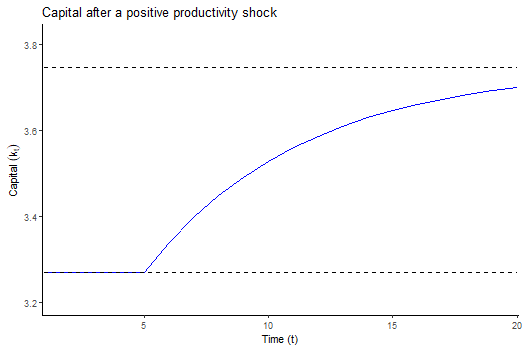
\includegraphics[scale=.6]{problem1_timeplot_k.png}
					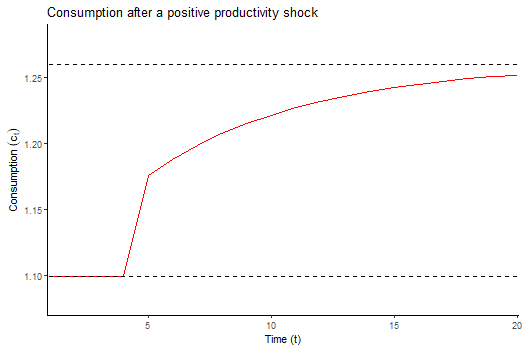
\includegraphics[scale=.6]{problem1_timeplot_c.png}
				\end{center}
				
			\item 
				\begin{enumerate}
					\item The charts below show the path using the direct recursive functions for $k_t$ and $c_t$. As you can see, the new steady state is not reached; capital explodes, leading to a decline in consumption.
						\begin{center}
							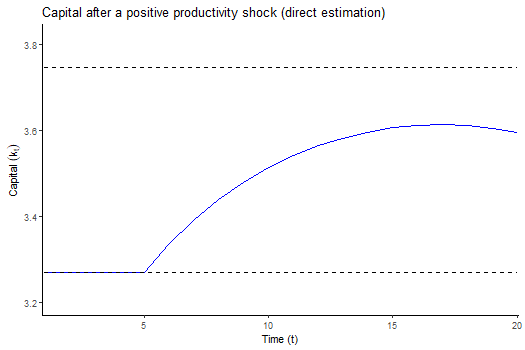
\includegraphics[scale=.6]{problem1.6_timeplot_k.png}
							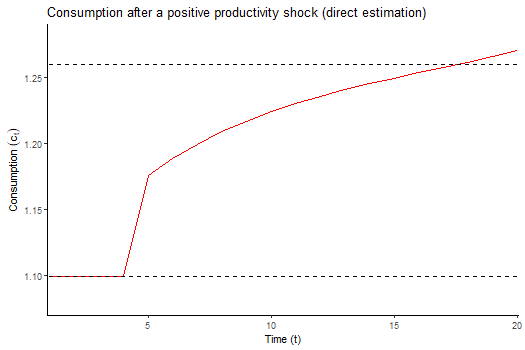
\includegraphics[scale=.6]{problem1.6_timeplot_c.png}
						\end{center}
						
					\item Using the "shooting method" yields $c_{t_0}=1.1742$. Direct estimation of $k_t$ and $c_t$ using this value appears to converge:
						\begin{center}
							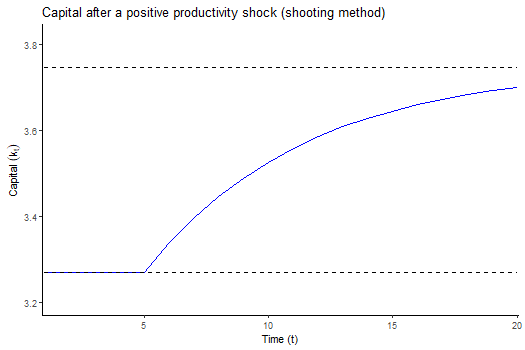
\includegraphics[scale=.6]{problem1.6b_timeplot_k.png}
							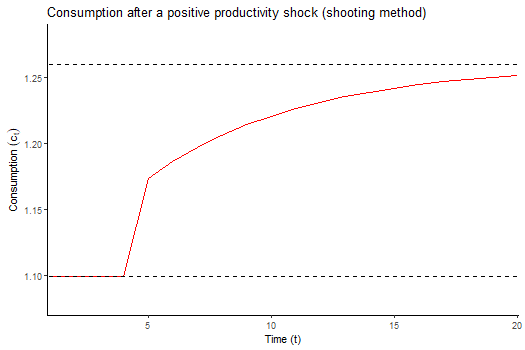
\includegraphics[scale=.6]{problem1.6b_timeplot_c.png}
						\end{center}
				\end{enumerate}
		\end{enumerate}
\end{enumerate}


%%%________________________________________________________________%%%

\section*{Question 2}
\textbf{In each of the environments below, state the Social Planner's Problem (SPP) and the Consumer Problem (CP), then define, but do not solve, the Competitive Equilibrium (CE).}
\medskip \\
\begin{itemize}
	\item[1.] \textbf{2-period overlapping generations problem}
		\medskip \\
		In each period, there are four agents in this model, with a four-element allocation, $\{c_t^{1t},c_t^{2t},c_t^{1t-1},c_t^{2t-1}\}$, where agents denoted with a superscript of 1 (type 1 agents) are endowed with $w_1$ when young, and type 2 agents are endowed with $w_2$ when old. There are $\frac{1}{2}N$ agents in each type so that there are $N$ agents in each generation. Let $N=1$ for notation purposes.
		\smallskip \\
		The social planner has access to $\frac{1}{2}w_1+\frac{1}{2}w_2$ in each period and weights all agents equally, with the problem:
		\begin{align*}
			&\underset{\{c_t^{1t},c_t^{2t},c_t^{1t-1},c_t^{2t-1}\}}{\text{max }}\text{ln}c_t^{1t}+\text{ln}c_t^{2t}+\text{ln}c_t^{1t-1}+\text{ln}c_t^{2t-1} \\
			&\text{  s.t.  }c_t^{1t}+c_t^{2t}+c_t^{1t-1}+c_t^{2t-1}\leq\frac{1}{2}w_1+\frac{1}{2}w_2
		\end{align*}
		In the decentralized economy with fiat currency, the money supply is fixed at $M$ with each (old) agent of generation $0$ given $M$ units of currency. Then there are four problems to solve in the decentralized economy: generation $0$, types $1$ and $2$, and generation $t$, types $1$ and $2$. In that order, the problems are:
		\begin{align*}
			&\underset{c_1^{10}}{\text{max }}\text{ln}c_1^{1,0}											 &\text{s.t. } &p_1c_1^{1,0}	\leq M 				\\
			&\underset{c_1^{20}}{\text{max }}\text{ln}c_1^{2,0}											 &\text{s.t. } &p_1c_1^{2,0}	\leq M + p_1 w_2	\\
			&\underset{\{c_t^{1t},c_{t+1}^{1t}\}}{\text{max }} \text{ln}c_t^{1t} + \text{ln}c_{t+1}^{1t}
				&\text{s.t. } 	&p_tc_t^{1t} + M^{1t}_{t+1}	\leq p_tw1\text{, }p_{t+1}c^{1t}_{t+1}		\leq M^{1t}_{t+1}	\\
			&\underset{\{c_t^{2t},c_{t+1}^{2t}\}}{\text{max }} \text{ln}c_t^{2t} + \text{ln}c_{t+1}^{2t}
				&\text{s.t. } 	&p_tc_t^{2t} + M^{2t}_{t+1}	\leq 0\text{, }p_{t+1}c^{2t}_{t+1}		\leq M^{2t}_{t+1}	
		\end{align*}
		In the competitive equilibrium, the goods and money markets clear:
		\begin{align*}
			c_t^{1t}+c_t^{2t}+c_t^{1t-1}+c_t^{2t-1} 		&= \frac{1}{2}w_1+\frac{1}{2}w_2	&\text{(Goods market)}	\\
			\frac{1}{2}M_{t+1}^{1t}+\frac{1}{2}M_{t+1}^{2t}	&= M								&\text{(Money market)}	
		\end{align*}
		
	\item[2.] \textbf{3-period overlapping generations problem}
		\medskip \\
		In each period, there are three agents, with a three-element allocation, $\{c_t^{t},c_t^{t-1},c_t^{t-2}\}$, and a total endowment of $N_{t-2}w_1+N_{t-1}w_2+N_tw_3=N_t(\frac{1}{n^2}w_1+\frac{1}{n}w_2+w_3$. The social planner's problem in each period, then, is:
		\[
			\underset{\{c_t^{t},c_t^{t-1},c_t^{t-2}\}}{\text{max }}\text{ln}c_t^{t}+\text{ln}c_t^{t-1}+\text{ln}c_t^{t-2}
				\text{ s.t. }c_t^t + \frac{1}{n}c_t^{t-1} + \frac{1}{n^2}c_t^{t-2} \leq \frac{1}{n^2}w_1+\frac{1}{n}w_2+w_3
		\]
		In the decentralized economy, the amount of fiat currency is fixed at $N_{-1}=\frac{1}{n^{t+1}}N_t$, which is evenly distributed to the initial old generation. There are three consumer problems: two in the initial period (old agents and middle-aged agents), and one in period $t$. These problems are provided below, in order the listed order.
		\begin{align*}
			&\underset{c_1^{-1}}{\text{max }}\text{ln}c_1^{-1}											 
				&\text{s.t. } &p_1c_1^{-1}	\leq \frac{1}{N_{-1}}+p_1w_3 							\\
			&\underset{\{c_1^0,c_2^0\}}{\text{max }}\text{ln}c_1^0+\text{ln}c_2^0						 
				&\text{s.t. } &p_1c_1^0+M_2^0 \leq p_1w_2\text{, }p_2c_2^0\leq p_2w_2 + M_2^0		\\
			&\underset{\{c_t^{t},c_{t+1}^{t},c_{t+2}^t\}}{\text{max }} \text{ln}c_t^{t} + \text{ln}c_{t+1}^{t} + \text{ln}c_{t+2}^{t}
				&\text{s.t. } 	&p_tc_t^t 			+ M^{t}_{t+1}	\leq p_tw1						\\
			&	&				&p_{t+1}c^t_{t+1}	+ M^{t}_{t+2}	\leq p_{t+1}w_2+M^{t}_{t+1}		\\
			&	&				&p_{t+2}c^t_{t+2}					\leq p_{t+2}w_3+M^{t}_{t+2}	
		\end{align*}
		In the competitive equilibirum, the goods and money markets clear:
		\begin{align*}
			c_t^{t}+\frac{1}{n}c_t^{t-1}+\frac{1}{n^2}c_t^{t-2}	&= w_1+\frac{1}{n}w_2++\frac{1}{n^2}w_3	&\text{(Goods market)}	\\
			M_{t+1}^{t}+\frac{1}{n}M_{t+1}^{t-1}				&= \frac{1}{n^{t+1}}					&\text{(Money market)}	
		\end{align*}
		
	\item \textbf{Cake eating problem}
		\medskip \\
		Our single agent faces the following problem at time $t$, which determines the agent's consumption in all subsequent periods:
		\[
			\underset{\{c_t\}_{t=1}^\infty}{\text{max }}\sum_{t=1}^\infty \beta u(c_t) \text{     s.t. }\sum_{t=1}^\infty c_t = k_1\text{, }c_t\geq 0\forall t
		\]
		
\end{itemize}


%%%________________________________________________________________%%%


\end{document}












